\chapter{Daten und Messungen}
\label{chap:dataandmeasure}

%%%%%%%%%%%%%%%%%%%%%%%%%%%%%%%%%%%%%%%%%%%%%%%%%%%%%%%%%%%%
\section{Mobile iBeacons}
\label{sec:dataandmeasurement:mobilebeacon}
%%%%%%%%%%%%%%%%%%%%%%%%%%%%%%%%%%%%%%%%%%%%%%%%%%%%%%%%%%%%
Die mobilen iBeacon verzichten, wie der Name schon andeutet, auf eine feste Stromquelle und werden ausschließlich mit Batterien betrieben.
Zum Einsatz kommen dabei die sogenannten Knopfzellen, welche mit einer Spannung von 3,0 Volt operieren.
Da Bluetooth Low Energy extrem energiesparend arbeitet, geben die Hersteller der Beacons, die Akkulaufzeit mit bis zu zwei Jahren, ohne einen Batteriewechel an. Diese Laufzeit hängt jedoch auch stark von der gewählten Signalstärke und dem gewählten Sendeinterval zusammen, welche die Laufzeit sehr stark beeinflussen können.

Bisher gibt es wenige Hersteller dieser iBeacons und der Großteil der Produkte befindet sich momentan noch in der Entwicklungsphase. Die genutzten iBeacons von \emph{estimote} und \emph{kontakt.io} sind ebenfalls noch in der Entwicklungsphase und hauptsächlich als Testgeräte für Entwickler ausgelegt. Dabei bleibt jedoch unklar in wie weit sich das fertige Produkt in den technischen Spezifikationen von den aktuellen Prototypen unterscheiden wird.

%%%%%%%%%%%%%%%%%%%%%%%%%%%%%%%%%%%%%%%%%%%%%%%%%%%%%%%%%%%%
\subsection{estimote Beacon}
\label{sec:dataandmeasurement:mobilebeacon:estimote}
%%%%%%%%%%%%%%%%%%%%%%%%%%%%%%%%%%%%%%%%%%%%%%%%%%%%%%%%%%%%
Die Firma \emph{estimote} mit Sitz in Polen, war ein der ersten, die ein funktionstüchtiges iBeacon vorgestellt haben und es in einem \emph{Developer Preview Kit} zum Verkauf anbieten.
Dieses Kit beinhaltet drei verschiedenfarbige Beacons, welche mit einer wiederverwendbaren Klebeschicht an der Unterseite ausgestattet sind. Dies erlaubt das beliebige Anbringen und Abziehen der Beacons auf allen glatten Oberflächen.
\begin{figure}[htb!]
		\centering
	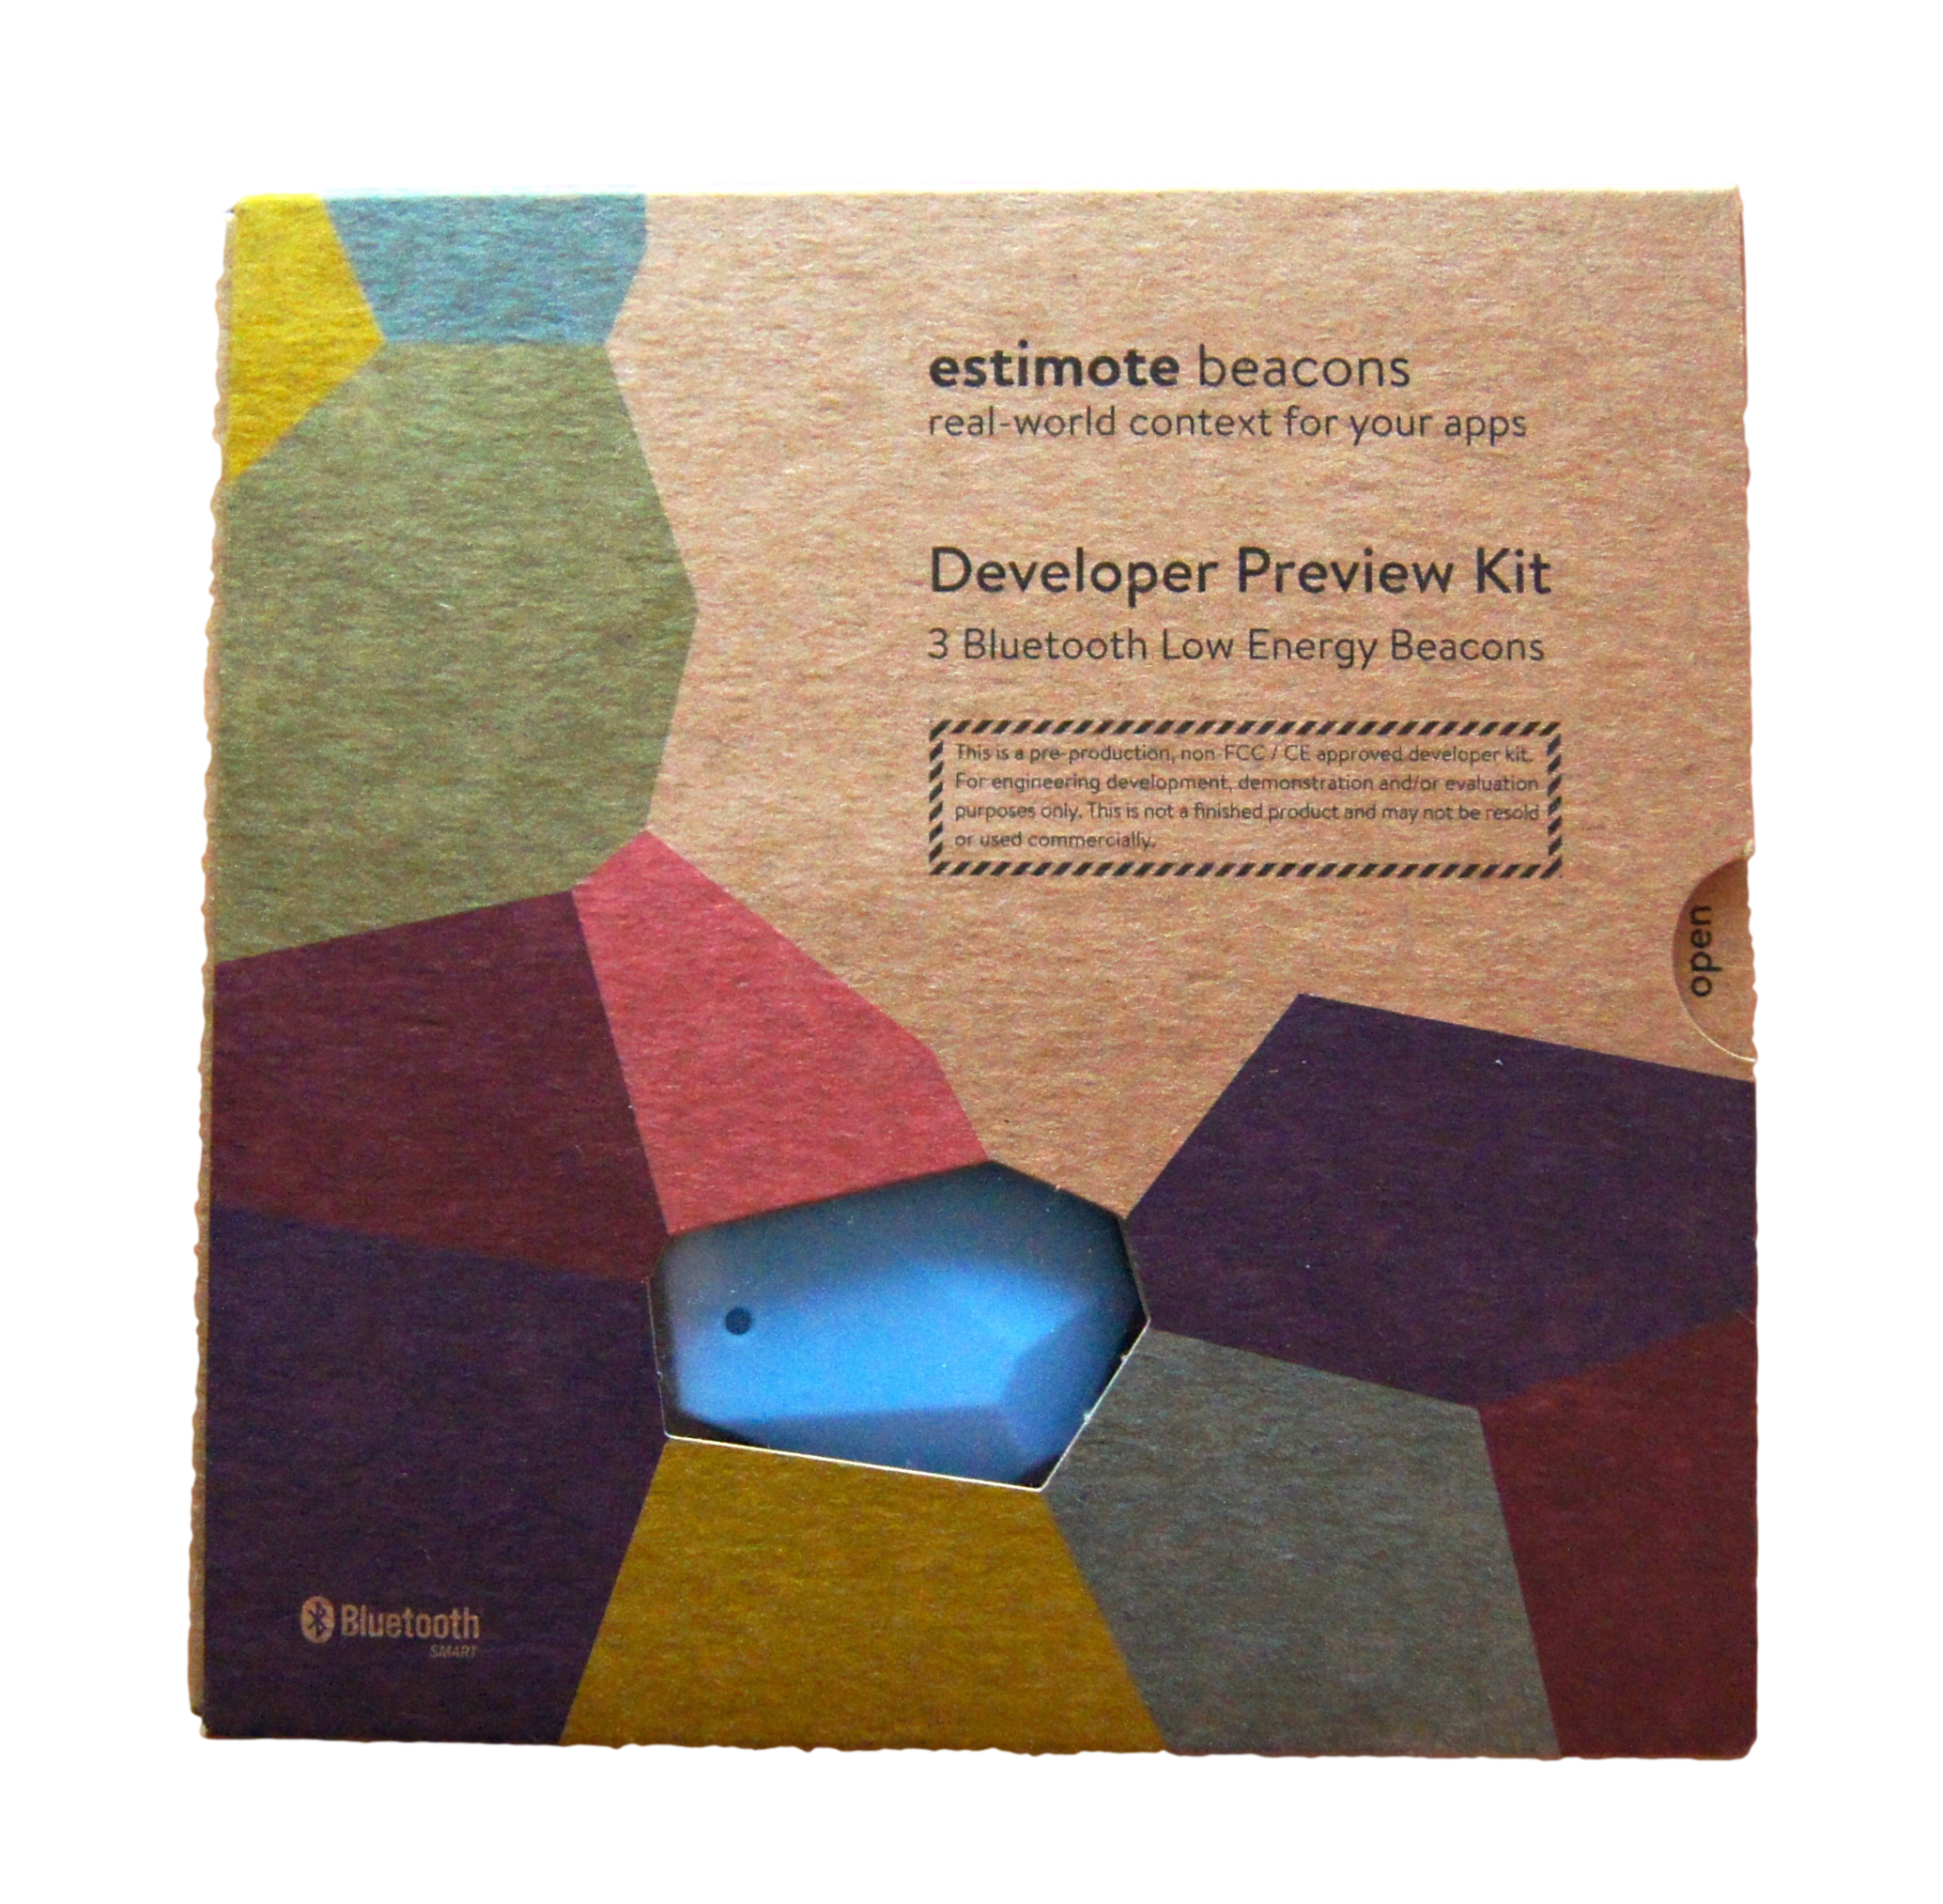
\includegraphics[scale=0.1]{estimote-developer-kit}
	\caption{Das Developer-Kit von estimote}
	\label{estimote-developer-kit}
\end{figure}

Im inneren des Beacons befindet sich ein Bluetooth Chipsatz von Nordic Semiconductor, welcher auf einem 32-bit ARM Prozessor beruht und mit einem 2,4Ghz Bluetooth Low Energy Modul arbeitet. Dabei verfügt der über 256 KB Flash-Speicher für Speicherung der Beacon-Konfiguration.
Speziell in den estimote-Beacon wurde dazu noch ein Temperatursensor eingebaut, welcher allerdings momentan noch nicht angesprochen werden kann.

Des Weiteren stellt estimote noch ein SDK für Android und iOS zur Verfügung, welches in Fall des iOS-SDK auf der iBeacons-API basiert, jedoch speziell auf die estimote-Beacons abgestimmt ist. 
Dabei bietet es neben den Funktionen der iBeacon-API noch die Funktionalität, sich mit den estimote Beacons zu verbinden und diese zu programmieren. So erlaubt es zum Beispiel die Signalstärke, das Sendeinterval und die Major-Minor-Informationen zu verändern oder die Firmware der Beacons zu aktualisieren.

Da das SDK, bis auf die Programmierung der Beacons, keine Vorteile gegenüber dem Core Location-Framework mit der iBeacons-API bietet, wurde jedoch auf die Verwendung verzichtet.

%%%%%%%%%%%%%%%%%%%%%%%%%%%%%%%%%%%%%%%%%%%%%%%%%%%%%%%%%%%%
\subsection{kontakt.io Beacon}
\label{sec:dataandmeasurement:mobilebeacon:kontaktio}
%%%%%%%%%%%%%%%%%%%%%%%%%%%%%%%%%%%%%%%%%%%%%%%%%%%%%%%%%%%%
Ein weiteres Unternehmen, welches sich eine eigene iBeacons-Lösung anbietet ist \emph{kontakt.io}. Auch hier ist noch kein finales Produkt erhältlich, sondern nur ein \emph{Dev Kit}, welches zehn Beacons enthält. 
Die Beacons sind relativ einfach gehalten und das Innere ist sehr einfach zugänglich, sodass ein Batteriewechsel sehr einfach ist.


\begin{figure}[htb!]
		\centering
	\includegraphics[scale=0.1]{kontakt-beacon-outside}
	\caption{Kontakt.io Beacon}
	\label{kontakt-beacon-outside}
\end{figure}

Die Beacons von \emph{kontakt.io} basieren dabei auf dem BLE113 Chipsatz von \emph{bluegiga}, welcher über 256 KB Flash-Speicher verfügt und über einen 8051 Mikrocontroller von Intel verfügt.


Auch kontakt.io bietet ein eigenes SDK an, welches im Gegensatz zu dem SDK von \emph{estimote} nicht nativ für die einzelnen Platformen entworfen wurde, sondern online über eine REST-Schnittstelle arbeitet.
Dabei stellt \emph{kontakt.io} ein Webpanel zur Verfügung, in welchem man die einzelnen Beacons mit ihrem UUID, Major und Minor-Wert registriert und jedem den jeweiligen Ort beziehungsweise die Funktion zuweisen kann. 


%%%%%%%%%%%%%%%%%%%%%%%%%%%%%%%%%%%%%%%%%%%%%%%%%%%%%%%%%%%%
\section{Stationäre iBeacons}
\label{sec:dataandmeasurement:stationarybeacon}
%%%%%%%%%%%%%%%%%%%%%%%%%%%%%%%%%%%%%%%%%%%%%%%%%%%%%%%%%%%%
Neben den mobilen iBeacons, welche mittels Batterien funktionieren, gibt es auch stationäre iBeacons, welche über eine stetige Anbindung an das Stromnetz angewiesen sind.
Dabei gibt es verschiedene Ansätze.
Zum einen bietet \emph{PayPal} einen Ansatz, bei dem die komplette Technik in einen USB-Stick integriert wird und dann über ein Standart USB-Netzteil an jeder Steckdose betrieben werden kann.

Eine andere Lösung ist die Nutzung eines Bluetooth 4.0-kompatiblen USB-Dongles an einem Computer. Dieser kann mit entsprechender Software zu einem iBeacon umfunktioniert werden.

%%%%%%%%%%%%%%%%%%%%%%%%%%%%%%%%%%%%%%%%%%%%%%%%%%%%%%%%%%%%
\subsection{Raspberry Pi als iBeacon}
\label{sec:dataandmeasurement:stationarybeacon:raspberrypi}
%%%%%%%%%%%%%%%%%%%%%%%%%%%%%%%%%%%%%%%%%%%%%%%%%%%%%%%%%%%%
Der Raspberry Pi ist ein Mini-Computer, welcher auf einem ARM-Prozessor basiert und als günstiger Computer für Programmiereinsteiger konzipiert wurde. Der kleine Computer ermöglicht aber auch andere Einsatzgebiete, zum Beispiel als Beacon.

Hierbei wurde eine Linux-Distribution auf dem Gerät installiert und als Bluetooth-Dongle kann ein Modul von \emph{Plugable Technologies} zum Einsatz, welches speziell Bluetooth 4.0 Unterstützung bietet.
Für die Umfunktionierung zum iBeacon wurde die Bluetooth-Software \emph{blueZ} eingesetzt, welche es erlaubt das Bluetooth-Modul anzusprechen und spezifische Nachrichten über Bluetooth zu schicken.
Diese Möglichkeit wurde von der Firma Radius Network vorgestellt, welche auch ein ausführliches Tutorial für die Nutzung des Raspberry Pi als iBeacon auf ihrer Webseite anbieten (\citet{radiusraspberry}).



%%%%%%%%%%%%%%%%%%%%%%%%%%%%%%%%%%%%%%%%%%%%%%%%%%%%%%%%%%%%
\section{Außenmessungen}
\label{sec:dataandmeasurement:outdoormeasure}
%%%%%%%%%%%%%%%%%%%%%%%%%%%%%%%%%%%%%%%%%%%%%%%%%%%%%%%%%%%%

%%%%%%%%%%%%%%%%%%%%%%%%%%%%%%%%%%%%%%%%%%%%%%%%%%%%%%%%%%%%
\section{Innenraummessungen}
\label{sec:dataandmeasurement:indoormeasure}
%%%%%%%%%%%%%%%%%%%%%%%%%%%%%%%%%%%%%%%%%%%%%%%%%%%%%%%%%%%%